\chapter{NG-HDMI-TS}
\label{chap:network-transmission}

% \section{仮説}
映像のIP伝送については既に多くの先行研究があり、映像を拠点間などで伝送するための製品なども存在している。

しかし、本論文では、拠点間のIP伝送だけにとどまらず、拠点内の設備までもをIP伝送することをテーマとしている。
拠点内の設備として、カメラやスイッチャー、ディスプレイなどの拠点内の設備までもをIP伝送で行う、Video over IP化にするというテーマである。

そのため、実際に制作の現場にIP伝送を普及させた際に、現在の伝送方法の課題が解決でき、IP伝送を利用することができるのかについて検証する。

% \subsection{Ethernetを活用するメリット}

\ref{chap:introduction}章で、述べた通り、ネットワークを活用することによって活かせるメリットは以下の3つである。

\begin{itemize}
  \item 1本のケーブルで複数や双方向の映像が可能
  \item 伝送スピードの向上
  \item コストダウン
\end{itemize}

しかし、Ethernetを利用するためにはデメリットがある

輻輳
導入コストの

また、映像伝送における重要なポイントは以下の3つである。

\begin{itemize}
  \item 画質、音質の劣化がない
  \item 伝送遅延を一定以下にする必要がある
  \item 安定性がある
\end{itemize}

また、IP伝送のメリットは以下の点である。

\begin{itemize}
  \item ユニキャスト、ブロードキャストが行える
\end{itemize}

これらの点において評価を行う。

\section{映像制作現場}

現在の映像制作現場には、カメラ、スイッチャー、ディスプレイなどをはじめとする多くの機器がある。
現在の中継現場における、機器同士の接続図を図\ref{fig:broadcast-diagram-on-sdi}に示す。
実際の中継現場では、映像の記録を行うためのレコーダー、映像の入出力を切り替えるためのルーター、その他の機器など必要ではあるが、ここでは割愛する。

\begin{figure}[htbp]
  \begin{center}
    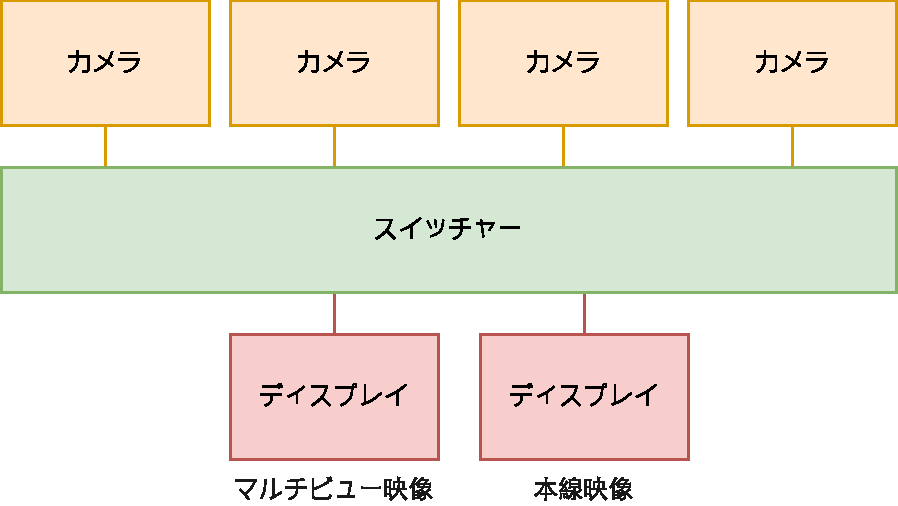
\includegraphics[bb=0 0 432 222,width=8.233cm]{img/broadcast-diagram-on-sdi.pdf}
  \end{center}
  \caption{現在の映像制作現場における機器同士の接続図}
  \label{fig:broadcast-diagram-on-sdi}
\end{figure}

4台のカメラを1台のスイッチャーに入力し、本線映像が出力される。
入力されたソースの映像が複数並んだマルチビュー映像を見てオペレーターが操作することが一般的である。
カメラとスイッチャー、スイッチャーとディスプレイは、それぞれSDIで伝送を行う。

Video over IP化が進んだ将来、理想的な中継現場における機器同士の接続図を図\ref{fig:broadcast-diagram-on-ip}に示す。

\begin{figure}[htbp]
  \begin{center}
    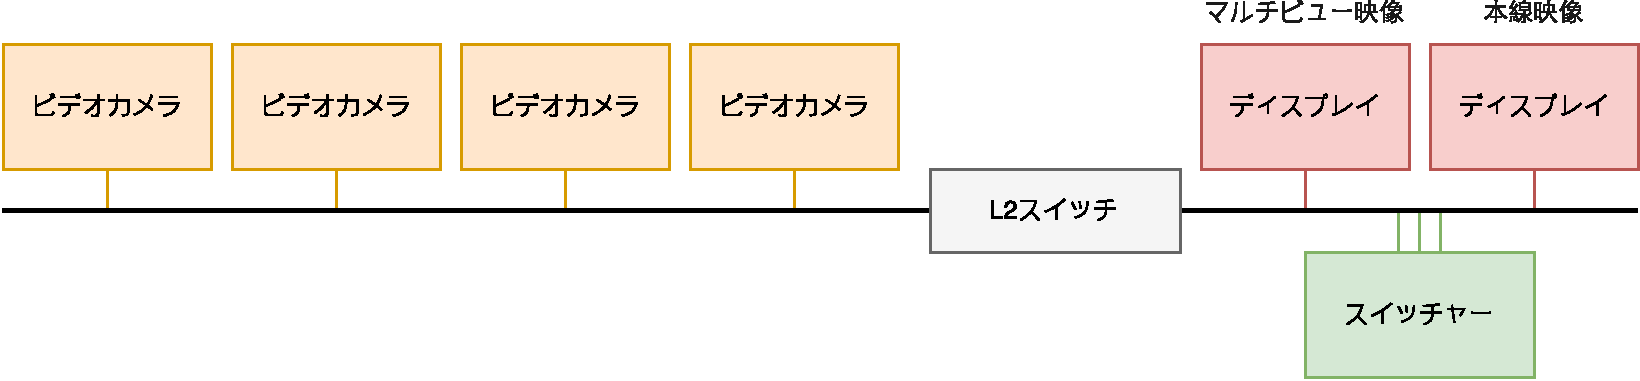
\includegraphics[bb=0 0 787 161,width=15cm]{img/broadcast-diagram-on-ip.pdf}
  \end{center}
  \caption{将来的な映像制作現場における機器同士の接続図}
  \label{fig:broadcast-diagram-on-ip}
\end{figure}

カメラとスイッチャー、スイッチャーとディスプレイは、それぞれIPで伝送を行う。
カメラからスイッチャーには1本の光ファイバーで接続されているが、スイッチャーからはソース映像、本線映像、マルチビュー映像のために3本の光ファイバーで接続されている。
設定解像度の使用する帯域によっては、1本で全ての映像を伝送できる場合もある。

\section{映像制作現場における遅延の許容値の調査}

映像制作現場において、オペーレーターが許容できる遅延の範囲を特定するため、遅延の許容範囲を調査する実験を行った。

ブラウザ上で、キーボードの入力を利用した擬似的なスイッチャーの操作を行い、マルチビュー映像の出力を行うプログラムを開発した。
プログラムで出力されるマルチビュー映像を図\ref{fig:mv-delay-virtual}のに示す。これは、実際の中継現場で利用されているマルチビュー映像とほぼ同じである。
実験では、$0ms$から$499.99ms$までを$33.33ms$間隔で分けた16段階のステップにわけて、各段階で入力から表示までの遅延を与える。
各段階で与える遅延については、心理的な判断を避けるため実験終了後まで表示を行わない。また、各段階で与える遅延は、実験ごとにランダムになっている。
各段階では、被験者からの入力を15秒間受け付ける。各段階の終了後、被験者に「遅延を許容できる」か「遅延を許容できない」かを問う。

この実験では、図\ref{fig:broadcast-diagram-on-ip}において、スイッチャーとマルチビュー映像を表示するためのディスプレイ間での遅延が許容できるかについて調査したことと同義である。

\begin{figure}[htbp]
  \begin{center}
    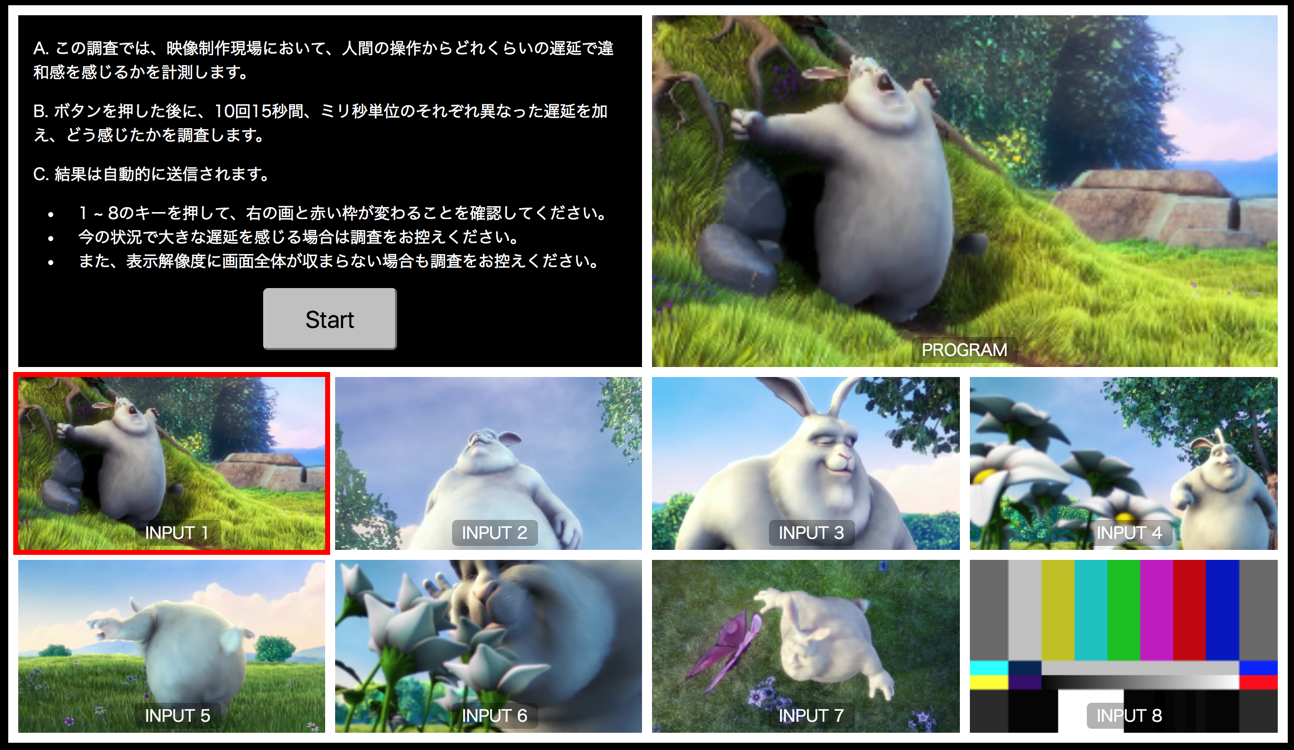
\includegraphics[bb=0 0 1294 750,width=14cm]{img/mv-delay-virtual.png}
  \end{center}
  \caption{今回の実験でWebページ上に再現したマルチビュー映像}
  \label{fig:mv-delay-virtual}
\end{figure}

\begin{figure}[htbp]
  \begin{center}
    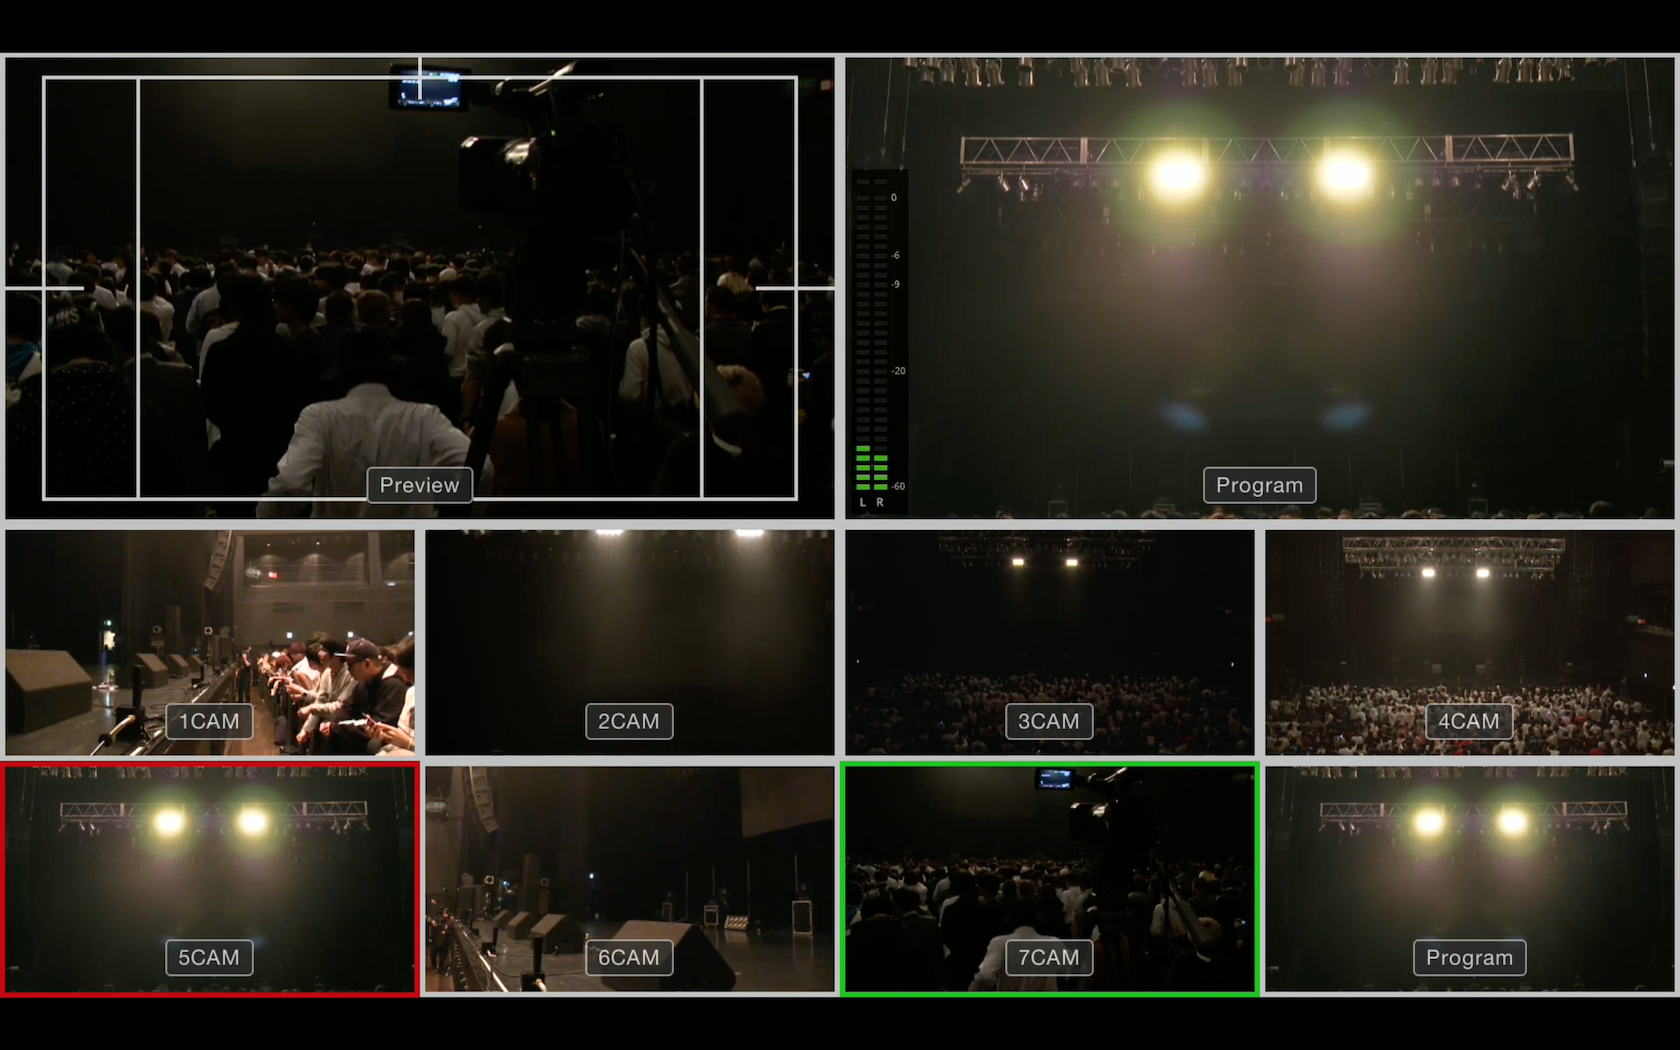
\includegraphics[bb=0 0 1680 1050,width=14cm]{img/mv-delay-actual.png}
  \end{center}
  \caption{実際の中継現場で利用されているマルチビュー映像}
  \label{fig:mv-delay-actual}
\end{figure}

実験では、ブラウザのレンダリング時間

\begin{table}[htbp]
  \caption{表}
  \label{tb:fpga-implement-modules}
  \begin{center}
  \begin{tabular}{r|l|l}
    \hline
    遅延時間(ミリ秒) & 遅延フレーム数 & 「遅延を許容できる」と回答した割合 \\\hline\hline
    0               & 0フレーム     & 97.56097561 \\\hline
    33.33           & 1フレーム     & 100         \\\hline
    66.66           & 2フレーム     & 97.56097561 \\\hline
    99.99           & 3フレーム     & 90.24390244 \\\hline
    133.33          & 4フレーム     & 90.24390244 \\\hline
    166.66          & 5フレーム     & 78.04878049 \\\hline
    199.99          & 6フレーム     & 75.6097561  \\\hline
    233.33          & 7フレーム     & 65.85365854 \\\hline
    266.66          & 8フレーム     & 46.34146341 \\\hline
    299.99          & 9フレーム     & 31.70731707 \\\hline
    333.33          & 10フレーム    & 27.5862069  \\\hline
    366.66          & 11フレーム    & 34.48275862 \\\hline
    399.99          & 12フレーム    & 34.48275862 \\\hline
    433.33          & 13フレーム    & 37.93103448 \\\hline
    466.66          & 14フレーム    & 34.48275862 \\\hline
    499.99          & 15フレーム    & 24.13793103 \\\hline
  \end{tabular}\end{center}
\end{table}


\begin{figure}[htbp]
  \begin{center}
    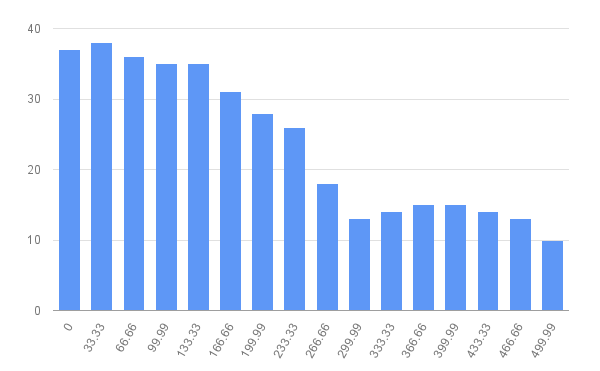
\includegraphics[bb=0 0 600 371,width=14cm]{img/mv-delay-result-graph.png}
  \end{center}
  \caption{グラフ}
  \label{fig:mv-delay-result-graph}
\end{figure}

\section{映像制作現場で求められるIP伝送装置の要件}
% ファイルベースの映像編集では、ネットワークストレージを活用した環境
% しかし、ライブでは、同軸ケーブルを利用してきました。これは、映像や音声を安定的に伝送することが求められているからです。

リアルタイムの映像伝送では、前出の通り同軸ケーブルを使用することが一般的である。

映像や音声を安定的に伝送することが出来、
現場での取り回しの氏易さ
IP

中継でのIP伝送では、ある程度の遅延[要出典]は許容することができる。
屋外での中継で、外にいるリポーターと局内にいるキャスターとの音声に遅延があり、やり取りに間があることがある。
これは、映像

しかし、拠点内でのIP伝送であれば、映像と音声が同期している必要があり、各カメラごとに遅延が異なるようではいけない。

\section{遅延}

\section{目的}

映像の制作の現場では、符号化・複合などによる映像の遅延を抑えることや、画質をそのまま伝送することがしばしば求められます。
このような背景から、4K映像を非圧縮のままIP伝送する技術の実証実験と、現場においてIP伝送を利用する際に問題となる点を洗い出します。?

% \section{構成}
